\chapter{Fundamentals}
\label{chap:fundamentals}

This chapter describes the fundamental basic standards that are used for Web and Enterprise Application Integration today that realized through service-oriented architectures often realized with Web service technologies.

Firstly, we provide some background about integration, integration middlewares and service-oriented architectures. Secondly, we introduce the general standards for service composition: choreography, behavioral interface and orchestration. Since, the thesis ideas based on the concept of Choreography, we will summarize the key papers that discover the choreography essence. Finally, as a prerequisite to formal theory, we present the description of communication behaviour through the Buyer-Seller-Shipper protocol.

\section{Integration technologies and their evolution}

Comprehensive enterprise-wide integration infrastructure usually requires more than one technology. Typically, also, because of the existing technologies, we will have to use a mixture of technologies. When selecting and mixing different technologies, we have to focus on their interoperability.

Interoperability between technologies is crucial because we will use them to implement the integration infrastructure. Achieving interoperability between technologies can be difficult even for technologies based on open standards. Small deviations from standards in products can deny the ``on-paper'' interoperability. For proprietary solutions, interoperability is even more difficult. Technologies used for integration are often referred to as middleware.

Middleware is system services software that executes between the operating system layer and the application layer and provides services. It connects two or more applications, thus providing connectivity and interoperability to the applications. The middleware concept, however, is today even more important for integration, and all integration projects will have to use one or many different middleware solutions. Middleware is mainly used to denote products that provide \textit{glue} between applications, which is distinct from simple data import and export functions that might be built into the applications themselves.

All forms of middleware are helpful in easing the communication between different software applications. The selection of middleware influences the application architecture, because middleware centralizes the software infrastructure and its deployment. Middleware introduces an abstraction layer in the system architecture and thus reduces the complexity considerably. On the other hand, each middleware product introduces a certain communication overhead into the system, which can influence performance, scalability, throughput, and other efficiency factors. This is important to consider when designing the integration architecture, particularly if our systems are mission critical, and are used by a large number of concurrent clients. There is a large variety of technologies existed today. The most common forms of middleware are:

\begin{enumerate}
\item  Message-oriented middleware

\item  Remote procedure calls

\item  Object request brockers

\item  Application servers

\item  Web services

\item  Enterprise service buses
\end{enumerate}

\subsection{Message-oriented middleware}

\begin{figure}
    \centering
    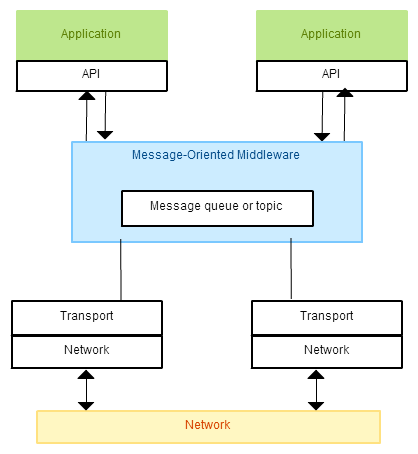
\includegraphics[width=0.8\textwidth]{resources/MOM.png}
    \caption{Message-oriented middleware}
    \label{fig:mom}
\end{figure}

Message-oriented middleware is a client / server infrastructure that enables and increases interoperability, flexibility, and portability of applications. It enables communication between applications over distributed and heterogeneous platforms. It reduces complexity because it hides the communication details and platform details. Usually the functionality of MOM is accessed via APIs. It provides asynchronous communication and uses message queues to store the messages temporarily. Therefore the interacted applications are loosely coupled. The messages can contain any type of data, asynchronous nature of communication enables the communication to continue even the receiver is temporary not available. The message waits in the queue and is delivered as soon as the receiver is able to accept it. The basic architecture is shown in the Figure \ref{fig:mom}. The well-known MOM technologies are RabbitMQ \cite{rabbitmq}, ZeroMQ \cite{zeromq}.

\subsection{Remote procedure calls}

Remote procedure calls are also a client / server infrastructure intended to enable and increase interoperability of applications over heterogeneous platforms. Similar to MOM, it enables communication between software on different platforms and hides almost all the details of communication. RPC is based on procedural concepts, such as developers use remote procedure or function calls.

\begin{figure}
    \centering
    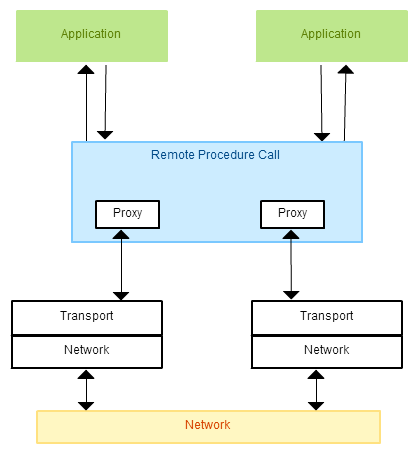
\includegraphics[width=0.8\textwidth]{resources/RPC.png}
    \caption{Remote Procedure Calls}
    \label{fig:rpc}
\end{figure}

RPC increases the flexibility of architecture by allowing a client of an application to employ a function call to access a server on a remote system. RPC allows the remote access without knowledge of the network address or any other lower-level information. The semantics of a remote call is the same whether or not the client and server are collocated. RPC is appropriate for client/server applications in which the client can issue a request and wait for the server to return a response before continuing with its own processing. On the other hand, RPC requires that the recipient is online to accept the remote call. If the recipient fails, the remote calls will not succeed, because the calls will not be temporarily stored and then forwarded to the recipient when it is available again, as is the case with MOM.

\subsection{Object request brockers}

Object request brokers (ORBs) are a middleware technology that manages and supports the communication between distributed objects or components. ORBs enable seamless interoperability between distributed objects and components without the need to worry about the details of communication. The implementation details of ORB are not visible to the components. ORBs provide location transparency, programming language transparency, protocol transparency, and operating system transparency.

\begin{figure}
    \centering
    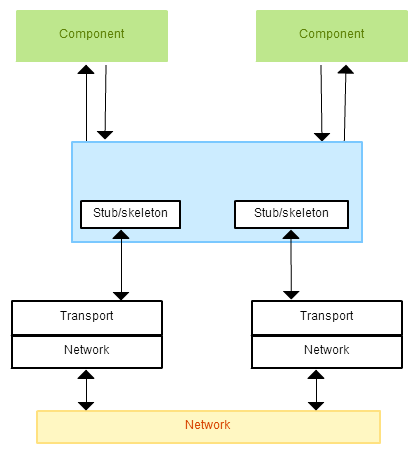
\includegraphics[width=0.8\textwidth]{resources/ORB.png}
    \caption{Basic ORB architecture}
    \label{fig:orb}
\end{figure}

The communication between distributed objects and components is based on interfaces. This enhances maintainability because the implementation details are hidden. The communication is usually synchronous, although is can also be deferred synchronous or asynchronous. ORBs are often connected with location services that enable locating the components in the network. ORBs are complex products but they manage to hide almost all complexity. More specifically, they provide the illusion of locality --- they make all the components appear to be local, while in reality they may be deployed anywhere in the network. This simplifies the development considerably but can have negative influence on performance. Figure \ref{fig:orb} depicts the basic ORB architecture. \cite{soaatoi}

ORB products may choose different scenarios as to how and where to implement their functionality. They can move some functions to the client and server components or they can provide them as a separate process or integrate them into to the operating system kernel. There are three major standards of ORBs:

\begin{compactenum}
\item  ORB CORBA

\item  Java RMI

\item  Microsoft COM/DCOM
\end{compactenum}

\subsection{Application servers}

Application servers handle the majority of interactions between the client tier and the data persistence tier. They provide a collection of already mentioned middleware services, together with the concept of a management environment in which we deploy business logic components --- the container. In the majority of application servers, we can find support for web services, ORBs, MOM, transaction management, security, load balancing, and resource management. Application servers provide a comprehensive solution to enterprise information needs. They are also an excellent platform for integration. Today, vendors often position their application servers as integration engines, or specialize their common purpose application severs by adding additional functionality, like connections to backend and legacy systems and position their products as integration servers. Although such servers can considerably ease the configuration of different middleware products, it is still worth thinking of what is underneath.

The application servers are software platforms, because it is a combination of software technologies necessary to run applications. In this sense, the application servers define the infrastructure of all applications developed and executed on them. Application servers can implement some custom platform, making them the proprietary solution of a specific vendor (these are sometimes referred to as proprietary frameworks). Such application servers are more and more rare.

\subsection{Web services}
Web services are the latest distributed technology that provides the technological foundation for achieving interoperability between applications using heterogeneous software platforms, operating systems, and programming languages. From the technological perspective, web services are the next evolutionary step in distributed architectures. Web services are similar to their predecessors, but also differ from them in several aspects.

Web services are the first distributed technology to be supported by all major software vendors. Therefore, it is the first technology that fulfills the universal interoperability promise between applications running on different platforms. The fundamental specifications that web services are based on are SOAP (Simple Object Access Protocol), WSDL (Web Services Description Language), and UDDI (Universal Description, Discovery, and Integration). SOAP, WSDL, and UDDI are XML based, making web services protocol messages and descriptions human readable.

From the architectural point of view, web services introduce several important changes compared to earlier distributed architectures. They support loose coupling through operations that exchange data only. This differs from component and distributed object models, where behavior can also be exchanged.

Operations in web services are based on the exchange of XML-formatted payloads. They are a collection of input, output, and fault messages. The combination of messages defines the type of operation (one-way, request/response, solicit response, or notification). 

Web services provide support for asynchronous as well as synchronous interactions. They introduce the notion of end-points and intermediaries. This allows new approaches to message processing. Web services are stateless and utilize standard Internet protocols such as HTTP (Hyper Text Transfer Protocol), SMTP (Simple Mail Transfer Protocol), FTP (File Transfer Protocol), and MIME (Multipurpose Internet Mail Extensions). So, connectivity through standard Internet connections is less problematic.

In addition to several advantages, web services also have a few disadvantages. One of them is performance, which is not as good as distributed architectures that use binary protocols for communication. The other is that plain web services do not offer infrastructure and quality of service (QoS) features, such as security, transactions, and others, which have been provided by component models for several years.

\subsection{Enterprise service buses}
An Enterprise Service Bus (ESB) is a software infrastructure acting as an intermediary layer of middleware that addresses the extended requirements that usually cannot be fulfilled by web services, such as integration between web services and other middleware technologies and products, higher level of dependency, robustness, and security, management, and control of services and their communication.

An ESB addresses these requirements and adds flexibility to communication between services, and simplifies the integration and reuse of services. An ESB makes it possible to connect services implemented in different technologies (such as EJBs, messaging systems, CORBA components, and legacy applications) in an easy way. An ESB can act as a mediator between different, often incompatible, protocols and middleware products.

The ESB provides a robust, dependable, secure, and scalable communication infrastructure between services. It also provides control over the communication and control over the use of services. It has message interception capabilities, which allow us to intercept requests to services and responses from services and apply additional processing to them. In this manner, the ESB acts as an intermediary.

An ESB usually provides routing feature to route the messages to different services based on their content, origin, or other attributes and transformation capability to transform messages before they are delivered to services. For XML-formatted messages, such transformations are usually done using XSLT (Extensible Stylesheet Language for Transformations) engine.

An ESB should make services broadly available. This means that it should be easy to find, connect, and use a service independently on the technology it is implemented in. With broad availability of services, an ESB can increase \textit{reuse} and can make the composition of services easier. Finally, an ESB should provide management capabilities, such as message routing, interaction, and transformation.

\section{Service-oriented architecture -- SOA}

\begin{figure}
    \centering
    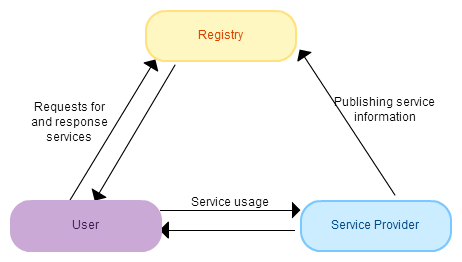
\includegraphics[width=0.8\textwidth]{resources/SOA.png}
    \caption{SOA components}
    \label{fig:soa}
\end{figure}

Services are the main concept of SOA. A service, as it is said, refers to an arbitrary piece of software that offers a well-defined function via standardized interfaces. A service can be reused by other services, legacy applications and customers. This requires that service interfaces and communication protocols must be platform independent. SOA services are loosely-coupled and can be reused whenever their functionality is required. An enterprise service-based architecture include a registry where all available services are listed. The list includes the general contracts of each service as well as technical description to invoke it. As Figure \ref{fig:soa} depicted, a SOA usually built on three main components: service providers and their services, a registry, and the service users. The service provider pushes the metadata of his services into the central point (registry). Then, user can search the services buy different criterias (metadata) and, as a result he gets a list of appropriate services and technical specification to invoke them.

Services should be designed according to tasks in business processes and form small and reusable units. Hence, a service possibly needs to access different databases or backend applications. So, this design criteria may be interpreted as a paradigm shift from solution islands, where one application exactly solves one problem.

Generally, nearly all programming languages or technologies for distributed systems can be used, because on a very high level of abstraction only the cross platform communication is a requisite. But in case the SOA should be interoperable, it is necessary that the communication is also independent from the service implementation. For example, Java RMI can be used to create a SOA although integration with other programming languages is difficult. Today, Web services are the de-facto standard used for the realization of SOAs. Such services use SOAP \cite{soap} and Internet protocols like HTTP for message exchange. Service descriptions are published using the Web Services Description Language (WSDL)  \cite{wsdlspec}. All these technologies are platform independent and enjoy significant support from the industry. Today, several proprietary and open-source frameworks are available as well as tools for Web service implementation and orchestration of Web services with WSDL and SOAP.

Besides SOAP-based Web services, also other communication protocols are used in modern SOAs, depending on the complexity and requirements. REST (Representation State Transfer) \cite{rest} services have become more and more popular during the last years because the protocol partly works without XML. REST communication is closely related to HTTP protocol, as it supports the following HTTP operations on stateful Web services. A resource is an object that represents the state of the service.

\begin{description}
\item[GET:] Requests the resource representation. The operation has no effect on the resource state.

\item[POST:] Adds and modifies a resource, since this can cause update on the persistence layer.

\item[PUT:] Creates new resources or replaces a resource.

\item[DELETE:] Deletes a resource.
\end{description}

In contrast to SOAP-based services, REST-ful service does not publish its interface in a standardized way. Instead, setting up a communication requires detailed knowledge about the interfaces. In compliance with the HTTP standard, parameters are submitted via the URL or as HTTP content -- normally as XML, JSON. The main advantage of REST services is its simplicity. It guarantees a high scalability because of a small software stack. However, the missing possibility for interface descriptions and the propagation of errors as HTTP error codes hamper a debugging of the communication compared to SOAP.

The loosely coupling of Web services offers various options for service combination as executable workflows. The most used techniques for workflow implementation are \textbf{service orchestration} and \textbf{service choreography} that we will talk about in the next sections of this chapter.  In short, service orchestration is the arrangement of service from a central instance, while service choreography routes messages in a peer-to-peer style directly between the participating services. In industrial scenarious, like the integration of information systems, service orchestration is preferred as a direct mapping of business processes to technical workflow descriptions and monitoring of business processes is possible.

To sum it up, a SOA is a paradigm to integrate different information systems and to integrate legacy systems. All components are implemented as loosely-coupled services. Through orchestration, informal business processes can be mapped to the technical system level. For example, workflows help to develop a consistent user interface that integrates several backend applications as a single service. The complexity of the involved interfaces in the backend communication is hidden transparently from the user client. Without SOA, the user would have to handle different application clients, each communicating with its own backend counterpart.

\section{General standards for service composition}

As it was mentioned in previous section, there is an increasingly widespread acceptance of SOA as a paradigm for integrating software applications within and across organizational boundaries. Therein, independently designed and operated applications are exposed as Web services. These services are further interconnected using an existing stack of standards including SOAP, WSDL, UDDI, etc. It is important to note, that the main open issue is in managing service interactions that go beyond simple sequences of requests and responses or involve large number of participants. Standardization is a key criteria of SOA. Such standardization initiates as WSDL, SOAP aim to ensuring interoperability between services developed on heterogeneous platforms. Figure \ref{fig:wsstd} provides a quick overview of existing WS standards. The standards in the category \textit{composition/processes} deal with the interplay between services and business processes. Today, there are two standardization initiatives: the Business Process Execution Language for Web Services (BPEL4WS or WS-BPEL) \cite{soaatoi} and the Web Services Choreography Description Language (WS-CDL) \cite{osw}. The significant attention raised by this category of standards discovers the fundamental links that exist between Business Process Management (BPM) and SOA. On the one hand, BPM techniques are used to resource management, process steps description, or capturing the interactions between a process and its environment. On the other hand, a service may serve as an entry point to an underlying business process.

There are three overlapping viewpoints exposed as the standards for service composition:

\begin{figure}
    \centering
    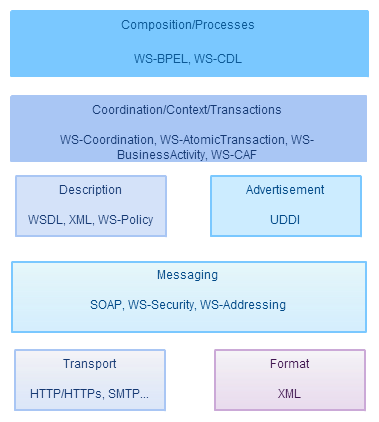
\includegraphics[width=0.8\textwidth]{resources/WS_stack.png}
    \caption{WS Standards}
    \label{fig:wsstd}
\end{figure}

Behavioural interface (abstract process in BPEL): It captures the behavioral dependencies between interactions in which specified service can engage.

Orchestration (executable process in BPEL): It deals with the description of the interactions in which a given service can engage with other services, as well as the internal steps between these interactions.

Choreography (multiparty collaboration in ebXML\footnote{Electronic Business using eXtensible Markup Language. Refer to \url{http://goo.gl/qw9hu}}): It describes collaborative processes involving multiple services where the interactions between these services are seen from the global viewpoint.

This thesis will focus on the choreography and behavioral interface viewpoints as a starting point for formal model of global description of interaction and local description of engaged participant. The following subsections provide more precise definitions of the above three viewpoints together.

\section{Choreography}

A \textit{choreography model} describes collaboration between a collection of services in order to achieve a common goal. It captures the interactions in which the participating services engage to achieve this goal and the dependencies between these interactions, including control-flow dependencies (a given interaction must occur before another one), data-flow dependencies, message correlations, time constraints, transactional dependencies, etc. A choreography does not describe any internal action that occurs within a participating service (local viewpoint) that does not directly result in an externally visible effect, such as an internal computation or data transformation. A choreography captures interactions from a global perspective, meaning that all participating services are treated equally. In other words, a choreography covers all the interactions between the participating services that are relevant with respect to its goal.

Figure \ref{fig:simplebsh} provides an example of a simple choreography through UML sequence diagram. Three services are involved in this choreography: one representing a \textit{buyer}, another one a \textit{seller}, and a third one a \textit{shipper}. The elementary actions in the diagram represent business activities that result in messages being sent or received. For instance, the action \textit{Request For Quote} undertaken by the buyer results in a message being sent to the seller; or depending on the decision of Buyer to accept or reject the quote, seller will continues or terminates the interaction. In addition, every message sending action has a corresponding message receipt action (dual interaction).

\begin{figure}
\centering
    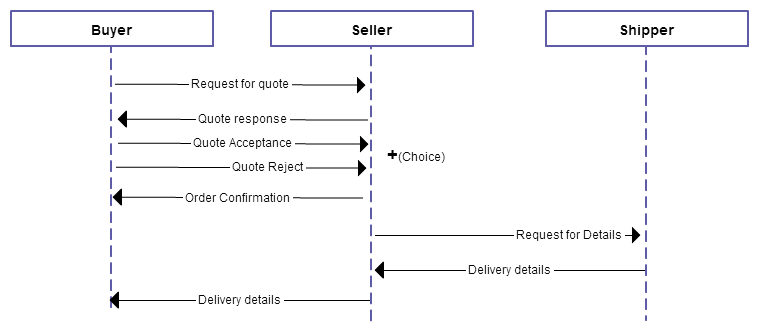
\includegraphics[width=0.8\textwidth]{resources/Choreography_bsh.png}
    \caption{Simple BSH protocol}
    \label{fig:simplebsh}
\end{figure}

In conclusion, a choreography constitutes an agreement (e.g. interface, contract) between a set of participants as to how a given communication should occur. This agreement may be established by common consultation or designed within a standardization committee.

\subsection{Behavioural interface}

A \textit{Behavioral interface model }captures the behavioral aspects of the interactions in which a particular service can engage to achieve a goal. It complements structural interface descriptions such as those supported by WSDL that capture the elementary interactions in which a service can engage, and the types of messages and the policies under which these messages are exchanged. A behavioral interface captures dependencies between interactions such as control-flow dependencies (e.g., that a given interaction must precede another one), data-flow dependencies, time constraints, message correlations, and transactional dependencies, etc.

Unlike a choreography, a behavioral interface focuses on the perspective of one single party. As a result, a behavioral interface does not capture \textit{complete interactions }since interactions necessarily involve two parties. Instead, a behavioral interface captures interactions from the perspective of one of the participants and can therefore be seen as consisting of communication actions performed by that participant. Like choreographies, behavioral interfaces do not describe internal tasks such as internal data transformations.

\begin{figure}
\centering
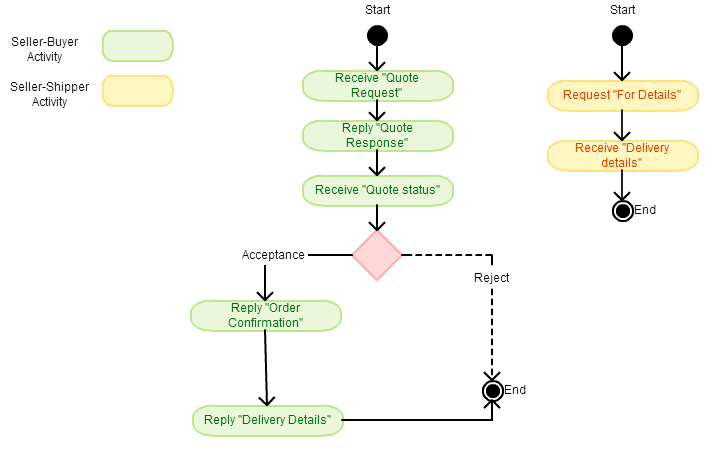
\includegraphics[width=0.8\textwidth]{resources/behav_interf_bsh.png}
\caption{Example of behavioural interface}
\label{fig:behavioural-interface}
\end{figure}

Figure \ref{fig:behavioural-interface} shows an example of behavioral interface using UML activity diagrams, where activities correspond to message sending and receipt. This behaviour interfaces cover behavior expected from the \textit{seller}'s role in the choreography of Figure \ref{fig:simplebsh}. The left behavioral interface reflects the \textit{seller-buyer }interaction, while the right one reflects the \textit{seller-shipper }interaction. 

The example illustrates the fact that in a given Business-to-Business (B2B) collaboration a role in a choreography may be associated with multiple behavioral interfaces. Moreover, given a choreography and a role within this choreography, an arbitrary number of behavioral interfaces may be defined that conform to the behavioral constraints imposed by the choreography on that particular role.

\subsection{Orchestration}

An \textit{orchestration model }describes both the communication actions and the internal actions in which a service engages. Internal actions include data transformations and invocations to internal software modules (e.g., \textit{legacy applications }that are not exposed as services). An orchestration may also contain communication actions or dependencies between communication actions that do not appear in any of the service's behavioral interface(s). This is because behavioral interfaces may be made available to external parties, and, thus, they should only show the information that actually needs to be visible to these parties. Orchestrations are also called \textit{executable processes }since they are intended to be executed by an \textit{orchestration engine}.

\begin{figure}
\centering
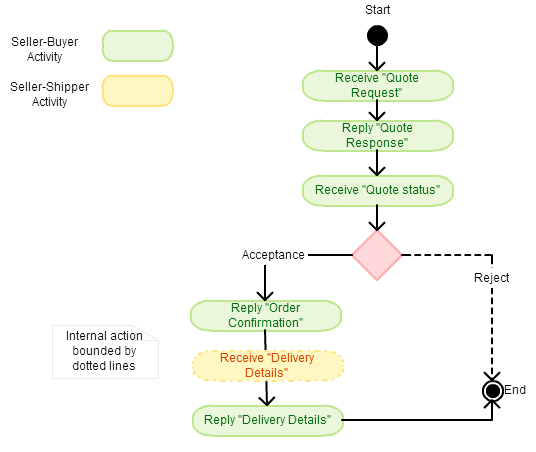
\includegraphics[width=0.8\textwidth]{resources/orchestration_internal_action.png}
\caption{Example of an orchestration in the form of an UML activity diagram}
\label{fig:orchestration-internal-action}
\end{figure}


Figure \ref{fig:orchestration-internal-action} shows an example of an orchestration in the form of an UML activity diagram. This orchestration adds an\textit{ internal action }(shown in dotted lines in the diagram) to the behavioral interface of Figure \ref{fig:behavioural-interface}.

The viewpoints presented above are overlap that exploited within service composition methodologies to perform consistency checks between viewpoints or to generate code. For example, a choreography model can be used for the following purposes:

\begin{compactenum}
\item  To generate the behavioral interface that each participating service must provide in order to participate in a collaboration. As explained below, this \textit{behavioral interface }can then be used during the development of the service in question.

\item  To check whether the behavioral interface of an existing service conforms to a choreography and, thus, whether the service in question would be able to play a given role in that choreography.
\end{compactenum}

Similarly, a behavioral interface may be used as a starting point to generate orchestration skeleton that can then be filled up with details, regarding internal tasks, and refined into a full orchestration. On the other hand, an existing orchestration can be checked for consistency against an existing behavioral interface. For example, it would be possible to detect the case where a given orchestration does not send messages in the order in which these are expected by other services.

\subsection{WS-CDL: issues and further actions}

The paper \cite{critical-ws-cdl} discovers the issues of the WS-CDL specification. Those issues become the starting point on my continuous research work.

So, one of the requirements of WS-CDL is to provide a means for tools to validate \textbf{conformance} to choreography descriptions to ensure \textbf{interoperability} between web services. To enable design time or static validation and verification of choreographies to ensure correctness properties such as livelock, deadlock, or to ensure that the runtime behavior of participants conforms to the choreography interface. WS-CDL must be \textbf{based on} a \textbf{formal language} that provide these validation capabilities.

The existing association between WS-CDL and WSDL is \textbf{too restrictive}. A choreography wired to specific WSDL interfaces (either indirectly through references to operations or more directly through an association between roles and their behaviors specified by reference to WSDL interfaces) cannot utilize functionally equivalent services with different WSDL interfaces. In other words, the choreography is statically bound to specific operation names and types, which may hinder the reusability of choreography descriptions. Cast more generally, choreography descriptions which abstractly describe behavior at a higher level, in terms of capability, would allow runtime selection of participants able to fulfill that capability, rather than restricting participation in the choreography to participants based on their implementation of a specific WSDL interface or WSDL operations.

A more subtle dependency is semantic consistency of a global choreography and local process orchestrations. Since a choreography definition introduces message ordering constraints over the interface views of local process orchestration definitions. These need to be supported at the orchestration level in which they are mapped. The expressive power of orchestration semantics, at the same time, should be not be limited by the choreography layer. \cite{critical-ws-cdl}

Also WS-CDL cannot conveniently support complex multi-party interactions without serializing it.

Finally, WS-CDL is an XML-based language standard. The development of a graphical language for capturing choreographies is not within the current choreography charter of W3C. Any exploitation of WS-CDL should be based on a graphical language, which supports user convenience in capturing specifications, model verification, and validation, as well as configuration for specific deployments utilizing different aspects messaging. Ultimately, it is worth remembering that choreography models are not intended to be directly executed. \cite{critical-ws-cdl}

\section{The essence of choreography}

Interacting processes must accomplish the goal of the computation. For this, the processes should have correct functionalities and correct interact with each other. With the interaction becoming more complex, the problems related to specify the interaction of the participants will be harder too, if we still want to do it locally.  In addition, it is harder to verify the interaction locally. These are the main motivation under the design of WS-CDL. Thus, a deeper understanding of the choreography is very important for the successful development of the web-based computation and application systems. It is better to be done at a suitable abstract level, to make a clear scenery of choreography \cite{essence-choreography}. The paper \cite{essence-choreography} defined a small language \textit{Chor}, a model of simplified WS-CDL, and a simple process language for the description of roles from a local viewpoint. Based on these models, the thesis discovers the concept of projections, that map a given choreography $C$ to a set of role processes. By extending a \textit{natural projection} to \textit{restricted natural choreography}, the paper \cite{essence-choreography} proposed another level of well-formedness.

Using a projection, we will get a set of processes, where each of them represents a role in the choreography. I studied the \textit{local conformance} problem in order to ask on the question: ``Does process $P$ can play role $R$ defined by choreography $C$?''.

So, a reasonable definition of the implementation of choreography is based on the concepts of \textit{projection} and \textit{local conformance}. By projection, it should be considered a procedure which takes a choreography in Chor and delivers and delivers a set of processes in the role language, while each of the processes corresponds to a role in choreography. In other words, a projection can partition a choreography into a set of processes which can mimic the behavior described by the choreography:

\begin{equation}
    \left[\left[\text{proj}\left(C,\ 1\right)||\dots || \text{proj}\left(C,\ n\right)\right]\right]=\ \left[\left[C\right]\right]
\end{equation}

As we will see in the next chapter \ref{chap:formal-theory} (``Formal Theory''), these processes make up an implementation of the choreography. 

The processes produced by natural projection cannot keep the relative order of their activities, thus, an extra trace of activities appears. So, in order to remedy the ordering problem, it must be inserted extra communication activities in the proper positions to synchronize these processes. The procedure inserts some communication activities in some positions of $C$, to produce, a revised choreography $C'$, such that we can ensure:

\begin{equation} 
[[\text{nproj}(C', 1) || \dots || \text{nproj}(C', n)]] |  \text{acts}(C) = \left[\left[C\right]\right]
\end{equation}

where $|$ is the filter operation.

\section{Main criterias for faultless web-services}

With a projection defined, it is easy to get a set of processes from a choreography which represent all the roles taking part in the task described by the choreography. In this section, I will turn to define the concept of the implementation of a role, e.g. if a process can play a role defined by choreography, it can take part in the choreography and play with the other valid roles.

The roles of a choreography define a set of requirements on a set of concrete processes (or, web services). In this case, when having a process at hand, we should have a way to decide if this process can play as a specific role. This is called the \textit{conformance }problem. It want to determine if a process conforms with a specific requirement expressed by a role. As said before, what was defined and discussed here can be named \textit{local conformance}, because it want to determine locally a relation between a role (requirement) and a process (a potential implementation). 

The following assumptions about a choreography are required to know:

\begin{compactenum}
\item  It describes all important roles taken part in the task. Each role should be implemented by an distinguishable independent process (an independent web-service) in the implementation. This also means that there should not be other substantial roles taking part in the interaction, except for the implementation of some local activities for some role(s).

\item  It describes all important message passing between the roles. The implementation should not add in other substantial interactions between roles, that is, no additional (substantial) message passing is allowed.

\item  The local activities described for each role are important. The implementation of a role (a process or a web-service) must perform the local activities of the specific role in a distinguishable way.
\end{compactenum}

Assume that a choreography \textit{C} defines random role \textit{R}, then a process \textit{P} may be considered as implementation of \textit{R}, $P \unrhd R$, if 

\begin{compactenum}
\item  \textit{P} can execute all communication required by \textit{R} with other roles of \textit{C}, in suitable time with suitable order.

\item  P support all the local activities mentioned in \textit{R}.
\end{compactenum}

\noindent The formal definitions and theorems are also presented in paper \cite{essence-choreography}.

\section{Why End-Point Projection (EPP) matters}

Why does EPP matter? First, with EPP we have a clear idea how a global description can be executed, and, therefore, its computational meaning is clear: \underbar{a central idea of web} \underbar{services}, or in general communication-centred programs and services, is that independently running concurrent agents achieve their application goals through their communication with each other. Thus a global description should be considered as describing behaviour of distributed communicating processes: the latter is the meaning of the former. In this sense, it is only when a uniform notion of EPP is given that the computational content of global descriptions is determined.

Second, EPP offers, for each end-point, what local behaviour a given global description specifies: if we wish to monitor whether an independently developed end-point program behaves in a way specified by a global description, then we can compare the former with the EPP of the latter. Or a programmer/designer working on each endpoint program can check whether it conforms to the original global description with respect to its communication behaviour (such validation, which we already defined as \textit{conformance validation}, will be particularly useful in collaborative program development).

Thirdly, EPP offer a central underpinning for the theoretical understanding of the structures of global description and their use. Indeed, EPP appears as a link of theories of processes and web service engineering. The established connection enables application of algebras, logics and types of theories of process calculi in the present engineering context. Web service engineering demands theoretical foundations because it is about \textbf{interoperability} among organizations with possibly conflicting interests and complex trust relationships that require a clear shared understanding on how they are to interact with each other in a given business protocol. We need a clear criteria as to whether each end-point (organization) is acting conforming to the protocol. It means, that we need clear engineering understanding backed up by a theoretical basis in order to conform the protocol to a regulation. 

Chapter \ref{chap:session-based-programming} provides a general framework for EPP, which can uniformly map a general class of global descriptions onto their end-point counterparts. 

The following three are natural formal criteria by which we can measure the effectiveness of an EPP scheme (which are in fact closely related to the two informal criteria we just noted). 

\begin{compactenum}
\item  Important, engineering criteria is that the resulting local descriptions have intuitively a clear and direct connection to the original global description. 

\item  It is also important to have a general and uniform scheme which can be applied to a large class of global descriptions.

\item  Mapping preserves types and other well-formedness conditions.

\item  The projected local description implements all behaviours expected from the original global description. Concretely, actions expected from a global description should be faithfully realized by communication among a collection of projected end-points. This property may be called \textit{completeness of EPP}.

\item  In the reverse direction, locally projected communicating processes should not exhibit observable behaviour not prescribed in global description, as far as its predefined interface goes.2 Concretely, communications among projected peers should not go beyond actions stipulated in the original global description. This may be called \textit{soundness of EPP.}
\end{compactenum}